\documentclass[conference]{IEEEtran}

\IEEEoverridecommandlockouts

\usepackage[T1]{fontenc}
\usepackage[utf8]{inputenc}
\usepackage{cite}
\usepackage{amsmath,amssymb,amsfonts}
\usepackage{graphicx}
\usepackage{booktabs}
\usepackage{multirow}
\usepackage{array}
\usepackage{url}
\usepackage{hyperref}
\usepackage{float}
\usepackage{algorithm}
\usepackage{algorithmic}
\usepackage{tikz}

\newcommand{\aeff}{\alpha_{\text{eff}}}
\newcommand{\abase}{\alpha_{\text{base}}}
\newcommand{\Rstar}{R^*}

\begin{document}

\title{Enhancing Cooperative Jamming for Physical Layer Security Under Imperfect Eavesdropper CSI via Uncertainty-Aware Soft Actor-Critic}

\author{
\IEEEauthorblockN{
M. Daniyal (2023406),
M. Afeef Bari (2023356),
Mahad Aqeel (2023286)
}
\IEEEauthorblockA{
CY315 --- Wireless and Mobile Security\\
Track 2: Implementation \& Optimization\\
GIK Institute of Engineering Sciences and Technology\\
Spring 2026
}
}

\maketitle

\begin{abstract}
Cooperative Friendly Jamming (CFJ) is a practical Physical Layer Security technique in which idle Access Points (APs) transmit artificial noise to suppress eavesdropper channels without dedicated hardware. Recent work has shown that Soft Actor-Critic (SAC)-based Deep Reinforcement Learning can effectively optimize AP transmit powers to maximize sum secrecy capacity in multi-AP Wi-Fi networks. However, every existing DRL-CFJ formulation assumes the agent is given the exact physical location of the eavesdropper at every timestep --- an assumption that cannot hold in practice, since passive eavesdroppers never transmit and therefore cannot be localized. In this paper, we port the Hoseini et al. CFJ framework from MATLAB to a reproducible Python/Gymnasium environment and propose Uncertainty-Aware SAC (UA-SAC), a modification to the SAC training loop that removes this assumption. UA-SAC replaces the single-sample reward with a worst-case reward over M sampled eavesdropper positions, augments the state with a normalized uncertainty variable $\rho$ that signals CSI quality to the agent, and scales the entropy coefficient with $\rho$ to broaden jamming coverage when location estimates are unreliable. Results show that UA-SAC achieves 3.10 bps/Hz sum secrecy capacity at maximum uncertainty --- a 32.5\% improvement over non-RL baselines and exceeding a perfect-CSI SAC agent despite having no knowledge of the eavesdropper's true location.
\end{abstract}

\section{Introduction}

Anyone near enough can pick up wireless signals because they spread out openly. Because of this exposure, encryption steps in - relying on complex math to protect data. However, managing keys adds delay and complexity, especially where devices lack power or speed \cite{wyner}. Instead of just locking messages, another method shapes how signals travel; it uses the physical environment to give authorized users an advantage over intruders. This design means secure communication becomes possible even if attackers have unlimited computing strength - as long as the right signal conditions exist \cite{wyner,gaussian,broadcast}.

One way to put physical layer security into practice is through Cooperative Friendly Jamming. When several access points share the same radio channel, ones that are not busy helping devices can send out tuned interference. That background signal makes it harder for eavesdroppers to catch data, yet people using the network nearby still get decent connections - thanks to proximity shielding them somewhat \cite{tekin,dong}. It works without special gear; regular Wi-Fi access points do fine if managed from one central spot \cite{wifi5,spectrum}. Figuring out just how loud each helper should broadcast remains tricky. Poor balance weakens security yet harms performance. Solving this gets harder fast when networks expand, leaving older techniques struggling to keep up \cite{hoseini}.

Starting off differently each time, Hoseini et al.~\cite{hoseini} turned CFJ power assignment into a Markov Decision Process; they applied Soft Actor-Critic methods \cite{sac1,sac2}. Their results showed reinforcement learning jams work better than even clever AP picks or spreading power evenly - this held true whether networks were small or large. Their work validated the DRL-CFJ paradigm. However, a critical limitation remains: the agent receives the exact $(x,y)$ coordinates of the eavesdropper as part of every observation. In any real deployment, passive eavesdroppers never transmit, so their location cannot be estimated. The sensitivity of PLS designs to eavesdropper CSI errors is well-documented in the MIMO beamforming literature \cite{mukherjee,wang}, yet this problem has not been addressed for DRL-based CFJ.

In this paper, we extend the work of \cite{hoseini} to the imperfect eavesdropper CSI setting. We first port the Hoseini et al. system to Python/Gymnasium as a reproducible open-source baseline. We then propose UA-SAC, which introduces three targeted modifications to the SAC training loop: a worst-case robust reward computed over M sampled eavesdropper positions per step, a normalized uncertainty variable $\rho$ added to the state so a single universal policy can adapt to all uncertainty levels, and $\rho$-scaled entropy regularization that broadens jamming coverage when the eavesdropper location estimate is unreliable. Unlike prior robust PLS designs that require full knowledge of the uncertainty bound \cite{mukherjee,wang}, UA-SAC requires only the operator's own sensor noise characterization --- a quantity that is always available regardless of whether the eavesdropper's location is known.

IRS-based PLS alternatives \cite{cui,yang} achieve comparable secrecy gains through passive beamforming but require dedicated reflective hardware. CFJ requires none and is deployable on existing infrastructure today \cite{wifi5,spectrum}.

The rest of the paper is structured as follows. Section II describes the system model and problem formulation. Section III presents the UA-SAC methodology. Section IV reports simulation results. Section V concludes the paper and outlines future directions.

\section{System Model}

We consider a downlink wireless network deployed in a $50\text{m} \times 50\text{m}$ area comprising $N=4$ Access Points, $K=2$ legitimate users, and $J=1$ passive eavesdropper. Node positions are randomized each episode. All APs share a single 2.4 GHz frequency band. APs assigned to a user transmit data; unassigned APs transmit jamming noise at a controller-optimized power level, forming the cooperative jamming structure of \cite{hoseini}. Since the network is centrally controlled via software \cite{wifi5,spectrum}, the locations of all APs and users are available to the controller. Eve is passive --- she never transmits, so her true location $E$ is never known to the controller and only a noisy estimate $\hat{E}$ is ever observed.

\begin{figure}[H]
    \centering
    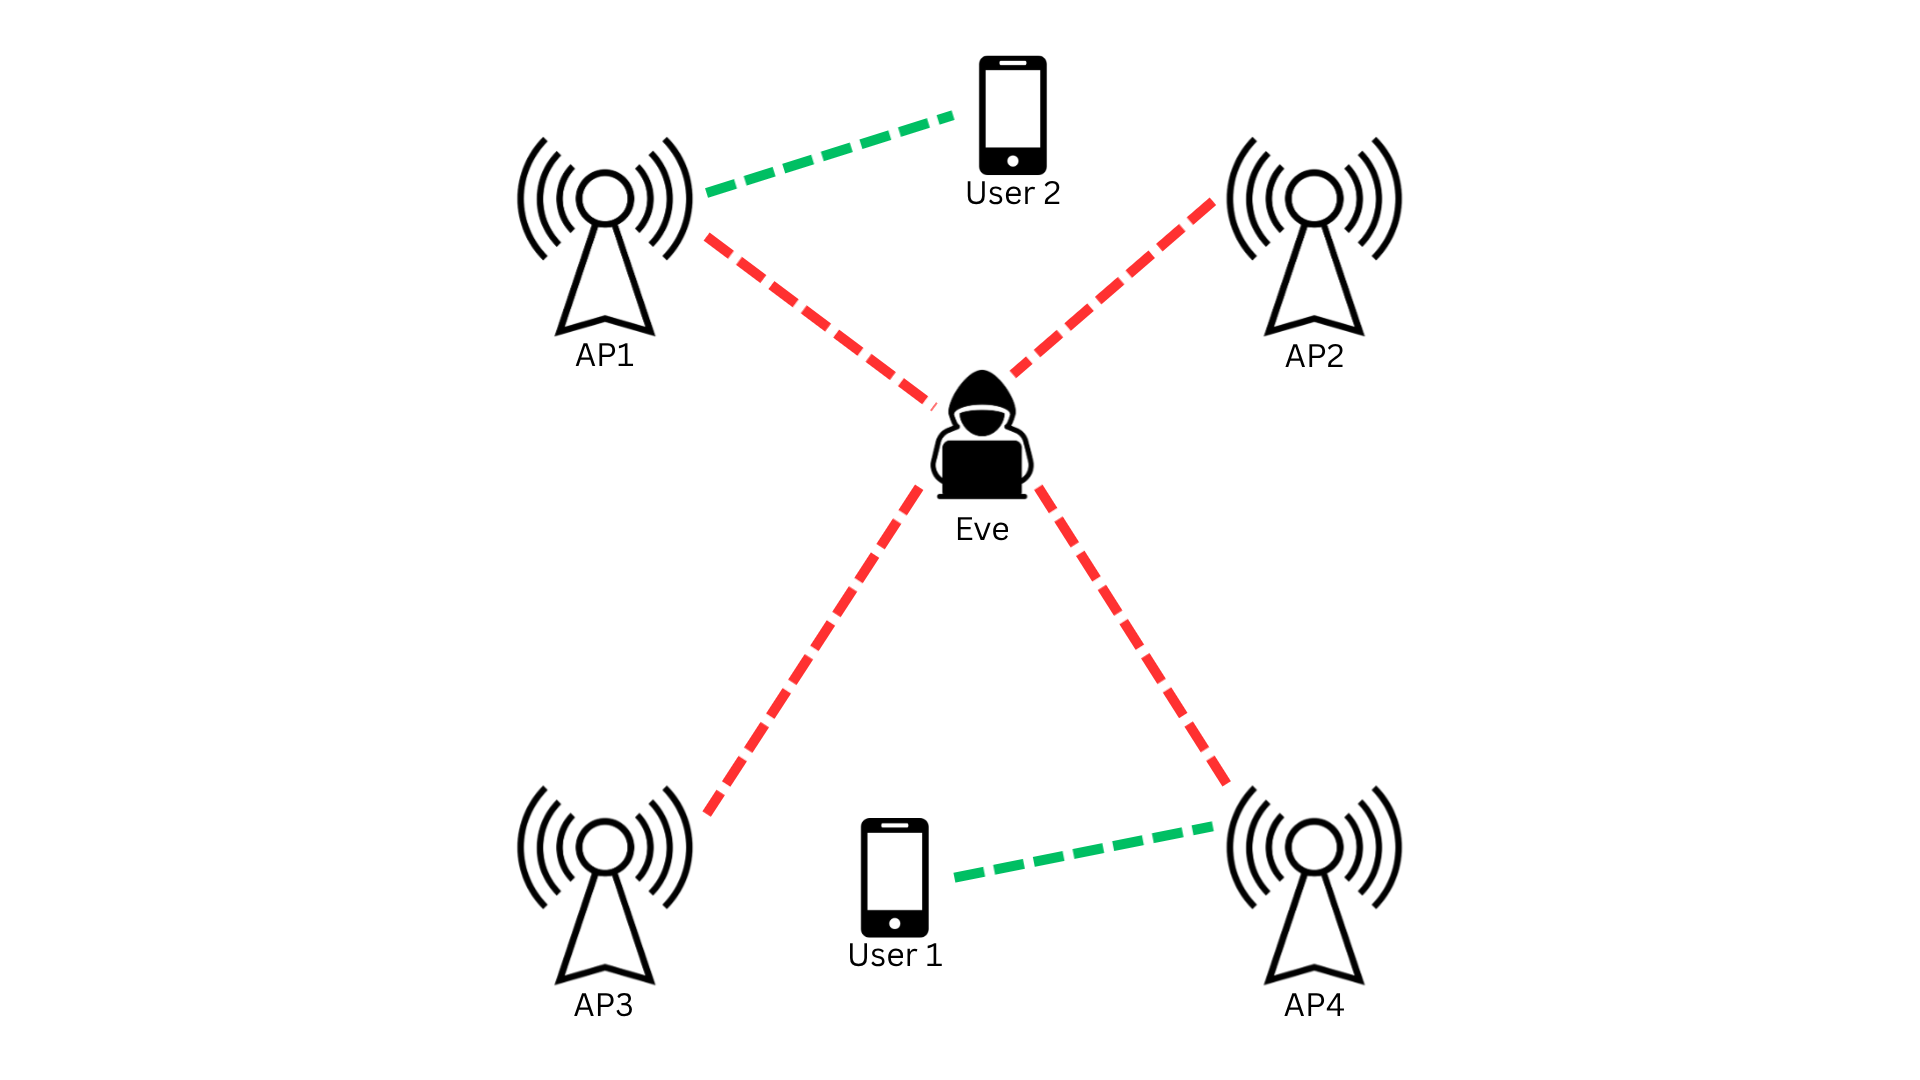
\includegraphics[width=\columnwidth]{AP1.png}
    \caption{System model illustrating the cooperative friendly jamming (CFJ) architecture with multiple APs, legitimate users, and a passive eavesdropper. User1 and user2 receive
traffic from AP1 and AP4, respectively (shown by green
dotted lines). However, Eve is eavesdropping on their
traffic (indicated by red dotted lines). Additionally, AP2 and AP3 are
idle and act as jammers.
}
    \label{fig:system_model}
\end{figure}

\subsection{Propagation Model}

We adopt the Friis free-space path loss model \cite{rappaport}. The received power at node $u$ from AP $n$ transmitting at power $p_n$ is

\begin{equation}
p^r_{n,u}=p_n\cdot\left(\frac{\lambda}{4\pi}\right)^2\cdot d_{n,u}^{-\gamma}
\end{equation}

where $d_{n,u}$ is the Euclidean distance between AP $n$ and node $u$, $\lambda=0.125$ m at $f=2.4$ GHz, and $\gamma=2.0$. The noise floor is $N_0=3.162\times10^{-12}$ W ($-85$ dBm), matching \cite{hoseini}. Antenna gains $G_t=G_r=1$ throughout.

\subsection{SINR and Channel Capacity}

The SINR at legitimate user $k$, served by AP $\alpha_k$, is

\begin{equation}
SINR_k=
\frac{p^r_{\alpha_k,k}}
{\sum_{n\neq\alpha_k}p^r_{n,k}+N_0}
\end{equation}

All APs --- whether serving another user or jamming --- contribute to the interference in (2). The Shannon capacity of the link between AP $n$ and user $k$ is

\begin{equation}
C_{n,k}=\log_2(1+SINR_{n,k})
\end{equation}

Similarly, the capacity of the channel between AP $n$ and eavesdropper $j$ is computed identically at Eve's coordinates:

\begin{equation}
C^e_{n,j}=\log_2(1+SINR_{n,j})
\end{equation}

where $SINR_{n,j}$ is the SINR at eavesdropper $j$ from AP $n$, with all other APs contributing interference. All capacities are in bps/Hz.

\subsection{Secrecy Capacity}

Assuming the worst-case eavesdropper has the highest capacity among all $J$ eavesdroppers wiretapping AP $n$:

\begin{equation}
C^e(n)=\max\{C^e_{n,j}:j=1,\dots,J\}
\end{equation}

The secrecy capacity for user $k$ associated with AP $\alpha_k$ is the non-negative excess of the legitimate link over the eavesdropper link \cite{wyner,gaussian,broadcast}:

\begin{equation}
C_s(u_k,\alpha_k)=
\left[C_{\alpha_k,k}-C^e(\alpha_k)\right]^+
\end{equation}

where $[x]^+=\max\{x,0\}$. A positive $C_s$ guarantees a coding scheme exists under which the eavesdropper cannot decode the message regardless of computational power.

\subsection{Problem Formulation}

The joint optimization over user association $A=[\alpha_1,\dots,\alpha_K]$ and transmit power $P=[p_1,\dots,p_N]$ is

\begin{equation}
\Psi:\max_{P,A}\sum_{k=1}^{K}C_s(u_k,\alpha_k),
\quad
\text{s.t. }0\leq p_n\leq P_{\max}
\end{equation}

Problem (7) is non-convex and jointly difficult. We decouple it into two subproblems following \cite{hoseini}. First, each user $u_k$ is associated with the AP that maximizes secrecy capacity under uniform maximum power:

\begin{equation}
\alpha_k=
\arg\max_n
C_s(u_k,n)\big|_{P=1\cdot P_{\max}}
\end{equation}

With association $A$ fixed, the remaining power allocation problem

\begin{equation}
\Phi:\max_{P}\sum_{k=1}^{K}C_s(u_k,\alpha_k),
\quad
\text{s.t. }0\leq p_n\leq P_{\max}
\end{equation}

is still non-convex, and we solve (9) with Deep Reinforcement Learning.

\begin{table}[t]
\caption{Simulation Parameters}
\centering
\begin{tabular}{|l|l|}
\hline
\textbf{Parameter} & \textbf{Value} \\
\hline
Area & $50\text{m} \times 50\text{m}$ \\
APs $(N)$ & 4 \\
Users $(K)$ & 2 \\
Eavesdroppers $(J)$ & 1 \\
Frequency & 2.4 GHz \\
Wavelength $\lambda$ & 0.125 m \\
Path loss exponent $\gamma$ & 2.0 \\
Noise floor $N_0$ & $-85$ dBm \\
Max transmit power $P_{\max}$ & 1.0 W \\
Episode type & Single-step \\
$\sigma$ (training) & $U[0,10]$ m per episode \\
$\rho=\sigma/D_{\max}$ & $[0,1]$ \\
Worst-case samples $M$ & 5 \\
Entropy scaling factor $\beta$ & 1.0 \\
\hline
\end{tabular}
\end{table}

\section{Literature Review}

Physical Layer Security as a formal discipline traces to Wyner's 1975 wiretap channel model \cite{wyner}, which established that secrecy is achievable without encryption when the legitimate channel has a structural advantage. The Gaussian wiretap extension \cite{gaussian} and multi-user generalization \cite{broadcast} followed, providing the capacity formulas this work builds on.

Cooperative jamming as a PLS mechanism was formalized by Tekin and Yener \cite{tekin} in the multi-access wiretap setting, and by Dong et al.~\cite{dong} for cooperative relay networks. Li et al.~\cite{iot} extended these ideas to IoT networks, sparking an interest in lean designs that reuse existing structures. While those studies set high-end performance limits, they stuck with fixed rules instead of learning on the fly.

Around 2018--2019, deep reinforcement learning started finding real footing in wireless network optimization. Luong et al.~\cite{luong} gave the field a broad map, covering how DRL applies across resource allocation, spectrum management, and routing, while Nasir and Guo~\cite{nasir} took a more targeted angle, deploying multiple cooperative agents to handle dynamic power demands in heterogeneous wireless environments. Li et al.~\cite{slice} applied the same family of methods to network slicing, demonstrating that learned policies could outperform static schedulers under variable traffic loads.

The present work adopts the Soft Actor-Critic algorithm~\cite{sac1,sac2}, consistent with Hoseini et al.~\cite{hoseini}. SAC's built-in entropy regularization discourages premature convergence to deterministic policies, a property that proves especially valuable when the operating environment shifts unpredictably, as it does when Eve's location is uncertain.

Robust beamforming under imperfect eavesdropper CSI has received sustained attention in the MIMO literature. Mukherjee and Swindlehurst~\cite{mukherjee} modeled CSI errors as norm-bounded uncertainty sets and derived worst-case beamformers accordingly. Wang et al.~\cite{wang} addressed a related problem with outage constraints on the legitimate link. Both works establish the principle of designing for the worst feasible Eve channel rather than the nominal one. We carry that principle into DRL-based CFJ, a setting where it has not previously appeared.

IRS-assisted physical layer security has also drawn growing attention~\cite{cui,yang}. Cui et al.~\cite{cui} showed that IRS phase shifts can be tuned to simultaneously focus energy toward intended receivers and scatter it away from eavesdroppers. CFJ takes a fundamentally different path: it exploits the access points already deployed in a Wi-Fi infrastructure~\cite{wifi5,spectrum}, requiring no additional hardware.

The direct foundation for this work is Hoseini et al.~\cite{hoseini}, who formulated CFJ power control as an RL problem in a multi-AP Wi-Fi setting and showed SAC-based allocation consistently outperforms fixed-power baselines. Their formulation assumed perfect knowledge of Eve's location, a gap they acknowledged but did not address. That gap is the starting point of what follows.

\section{Proposed Methodology}

Casting equation (9) as an MDP, we solve it with SAC~\cite{sac1,sac2}, extending the framework of~\cite{hoseini}. Where~\cite{hoseini} assumes exact eavesdropper positions, UA-SAC departs from that in three concrete ways.

\subsection{UA-SAC}

\subsubsection{Layer 1 --- Worst-Case Robust Reward}

In \cite{hoseini}, they figure the reward using just one precise spot for Eve. Instead, we use the lowest score across five separate fuzzy positions each time we train:

\begin{equation}
\hat{E}_i=
\text{clip}(E+\epsilon_i,0,D_{\max}),
\quad
\epsilon_i\sim\mathcal{N}(0,\sigma^2I_2)
\end{equation}

The reward is the minimum secrecy across all $M$ samples:

\begin{equation}
R^*=
\min_{i=1}^{M}
\sum_{k=1}^{K}
\left[
C(AP_{\alpha_k}\rightarrow u_k|P)
-
\max_j C(AP_{\alpha_k}\rightarrow e_j|P,\hat{E}_i)
\right]^+
\end{equation}

\subsubsection{Layer 2 --- Uncertainty-Augmented State}

We introduce a normalized uncertainty ratio:

\begin{equation}
\rho=\sigma/D_{\max}\in[0,1]
\end{equation}

The augmented state is:

\begin{equation}
s^*=
[
x_1,y_1,\dots,x_4,y_4
|
x_{u_1},y_{u_1},x_{u_2},y_{u_2}
|
\hat{e}_x,\hat{e}_y
|
\rho
]
\in\mathbb{R}^{15}
\end{equation}

Each episode picks a random $\sigma\in[0,10]$ meters. The action space is the continuous transmit power vector:

\begin{equation}
P=[p_1,p_2,p_3,p_4],
\quad
p_n\in[0,P_{\max}]
\end{equation}

\subsubsection{Layer 3 --- Uncertainty-Scaled Entropy}

The SAC entropy coefficient is scaled linearly with $\rho$:

\begin{equation}
\alpha_{\text{eff}}(\rho)=
\alpha_{\text{base}}
\cdot
(1+\beta\cdot\rho),
\quad
\beta=1.0
\end{equation}

\subsection{UA-SAC Formulation}

The complete UA-SAC optimization problem is:

\begin{equation}
\Phi_{UA}:
\max_P
\mathbb{E}_{\sigma\sim U[0,10]}
[R^*(s^*,\pi_\theta)],
\quad
\text{s.t. }
0\leq p_n\leq P_{\max},
\;
\rho=\sigma/D_{\max}
\end{equation}

The full training objective is:

\begin{equation}
J_{UA}(\pi_\theta)=
\mathbb{E}_{s^*\sim D}
\left[
R^*(s^*,\pi_\theta(s^*))
+
\alpha_{\text{base}}
(1+\beta\cdot\rho)
H(\pi_\theta(\cdot|s^*))
\right]
\end{equation}

\subsection{UA-SAC Algorithm}

\begin{algorithm}[H]
\caption{UA-SAC: Uncertainty-Aware Soft Actor-Critic}
\begin{algorithmic}[1]
\STATE \textbf{Initialize:} neural network policy $\pi_\theta$, two critics $Q_\phi$, replay buffer $\mathcal{B}$
\FOR{each episode}
    \STATE Place APs, users, and Eve randomly in the $50\text{m} \times 50\text{m}$ grid
    \STATE Draw uncertainty level: $\sigma \sim \mathcal{U}(0, 10\text{m})$, set $\rho = \sigma / D_{\max}$
    \STATE Perturb Eve's location by Gaussian noise to get $\hat{E}$ \hfill \textit{(agent never sees true $E$)}
    \STATE Form state: $s^* = [\,\text{AP positions} \mid \text{user positions} \mid \hat{E} \mid \rho\,] \in \mathbb{R}^{15}$
    \STATE Agent selects AP transmit powers: $P = \pi_\theta(s^*)$
    \STATE Sample $M=5$ plausible Eve locations $\{\hat{E}_1,\ldots,\hat{E}_5\}$ around true $E$
    \STATE Compute $\Rstar = \min_i \sum_k C_s(u_k \mid P, \hat{E}_i)$ \hfill \textit{(worst-case secrecy)}
    \STATE Store $(s^*, P, \Rstar)$ in buffer $\mathcal{B}$; sample a random minibatch
    \STATE Scale entropy: $\aeff = \abase \cdot (1 + \beta\rho)$ \hfill \textit{(higher $\rho$ = explore more)}
    \STATE Update critics and policy using standard SAC updates with $\aeff$
\ENDFOR
\end{algorithmic}
\end{algorithm}

\subsection{Implementation}

The full environment is implemented as a Gymnasium environment (\texttt{env/cfj\_env.py}) with Stable-Baselines3 SAC and trained over 100,000 timesteps using 4 parallel environments (\texttt{SubprocVecEnv}).

\section{Results and Discussion}

Evaluation used 1,000 fixed-seed randomized topologies. All agents are evaluated against the true eavesdropper location during testing.

\subsection{Training Convergence}

Figure~\ref{fig:training_convergence} shows the UA-SAC worst-case reward $R^*$ over 25,000 training episodes. $R^*$ rises from approximately 1.8 bps/Hz in early training to a peak of 2.75 bps/Hz, with a clear upward trend throughout. Episode-by-episode variance is high because $\sigma$ is randomized each episode --- easy episodes ($\rho \approx 0$) and hard episodes ($\rho \approx 0.2$) are interleaved in the same training stream. Upward movement continues, showing how the approach adapts by lifting performance even under toughest conditions, rather than just excelling in simpler setups.

\begin{figure}[H]
    \centering
    \includegraphics[width=\columnwidth]{uasac_convergence.png}
    \caption{UA-SAC training convergence showing worst-case reward $R^*$ versus training episodes.}
    \label{fig:training_convergence}
\end{figure}
\subsection{System Comparison at $\sigma=10$m}

Every system hits full secrecy when things get shaky ($\sigma = 10$m), according to Table~\ref{table:comparison_sigma10}. Each one clocks a perfect score on secrecy ratio, no exceptions. Because of this, doubt fades --- the CFJ trick works for everyone, even if power settings stay flat. The success does not shift itself, but how rich the outcome gets across setups shifts.

\begin{table}[htbp]
\caption{System Comparison at $\sigma = 10$m}
\label{table:comparison_sigma10}
\centering
\begin{tabular}{@{}lccc@{}}
\toprule
\textbf{System} &
\textbf{\begin{tabular}[c]{@{}c@{}}Sum Secrecy \\ (bps/Hz)\end{tabular}} &
\textbf{\begin{tabular}[c]{@{}c@{}}Gain over \\ Fixed Power\end{tabular}} &
\textbf{\begin{tabular}[c]{@{}c@{}}Secrecy \\ Ratio\end{tabular}} \\
\midrule
Fixed Max Power (no RL)    & 2.34 & ---    & 100\% \\
Baseline SAC (perfect CSI) & 2.98 & +27.4\% & 100\% \\
UA-SAC (ours)              & 3.10 & +32.5\% & 100\% \\
\bottomrule
\end{tabular}
\end{table}

It is interesting how UA-SAC hits 3.10 bps/Hz when $\sigma$ equals ten meters --- beating the baseline SAC even without knowing where Eve really hides. That edge comes from equation (11)'s harsh rule: aim for lowest secrecy among many fake Eve spots every update, pushing UA-SAC to spend power like it expects betrayal. Meanwhile, regular SAC learned solely on clean data, zero noise, so real-world fuzz trips it up hard during actual use.

\begin{figure}[H]
\centering
\includegraphics[width=1\linewidth]{plot1.png}
\caption{Three-system bar chart showing sum secrecy capacity and secrecy ratio at $\sigma = 10$m.}
\label{fig:comparison_bar}
\end{figure}

\subsection{Secrecy Capacity vs. CSI Uncertainty}
The graph displays average secure transmission rates at eleven different noise settings, ranging from zero to ten meters. When there is no added distortion, UA-SAC does slightly better than standard SAC - achieving 3.13 instead of 3.02 bits per second per hertz - since its learning process includes varying noise conditions and prepares it for tougher scenarios. With increasing interference, regular SAC performs worse over time due to reliance on precise eavesdropper positions without ability to adjust when those become uncertain. In contrast, UA-SAC holds steady throughout all distortions; it receives real-time cues about how much uncertainty exists through variable $\rho$ in equation (12), while its training objective in equation (11) already exposes it to every possible noise intensity. Every now and then, a quiet hum stays constant - CFJ stuck, regular Wi-Fi too, both flat at 2.34 bps/Hz across the board. Since neither one pays attention to where Eve might be, confusion changes nothing. Watch closely - the two learning systems hover higher, no matter how much static blurs the air.
\begin{figure}[H]
\centering

\includegraphics[width=1\linewidth]{plot2_secrecy_vs_noise.png}
\caption{Mean secrecy capacity vs. $\sigma$ for four systems.}
\label{fig:secrecy_vs_noise}
\end{figure}

\subsection{Normalized Robustness}

At $\sigma = 0$, each RL agent is set to $100\%$, making it easier to observe how performance degrades as noise increases. When $\sigma$ rises, performance declines occur, although not equally across agents. UA-SAC holds up well under increasing uncertainty; at $\sigma = 10\,\mathrm{m}$ it still achieves $99.0\%$, a negligible drop from its $\sigma = 0$ baseline. Standard SAC lands at $98.5\%$ under the same conditions. The raw numbers look close, but what they reflect is not. Both curves start at the same point when $\sigma = 0$, and the separation widens steadily as noise increases, with each step adding to standard SAC's disadvantage.

This behavior traces directly back to Equation~(11). Training against worst-case Eve signal selections, taken via minimization over $M$ realizations, costs the agent a marginal amount under clean conditions but pays back considerably when conditions turn adversarial. A slight dip at the peak is the price; what is gained in return is a policy that degrades more slowly as uncertainty grows. Prior robust secure communication work~\cite{mukherjee,wang} operated on similar logic, though in those cases robustness was baked into the beamformer design. Here it lives inside the learned transmission policy itself.

\begin{figure}[H]
\centering
\begin{tikzpicture}
    \node[anchor=south west, inner sep=0] (image) at (0,0) {
        \includegraphics[width=\linewidth]{plot3_robustness.png}
    };
    \node[font=\tiny, text=blue] at (8, -0.1) {$-1.5\%$};
\end{tikzpicture}
\caption{Normalized robustness versus CSI uncertainty $\sigma$ for SAC and UA-SAC.}
\label{fig:robustness}
\end{figure}

\subsection{Entropy Coefficient Evolution}

Figure~\ref{fig:entropy_evolution} tracks $\alpha_{\mathrm{base}}$, automatically tuned by SAC, alongside $\alpha_{\mathrm{eff}} = \alpha_{\mathrm{base}} \cdot (1 + \beta \rho)$ across $25{,}000$ gradient steps, with the mean batch value $\bar{\rho} \approx 0.10$ plotted on the secondary axis. Both coefficients open near $1.0$ and fall sharply, settling close to zero by step $10{,}000$ as the policy converges. Throughout training, $\alpha_{\mathrm{eff}}$ remains higher than $\alpha_{\mathrm{base}}$, with the difference determined by the average value of $\rho$ across batches, as defined in Equation~(15). The shaded region between the two curves --- largest during the early training phase where exploration is most important --- represents the uncertainty boost $\Delta \alpha$ applied by UA-SAC. This confirms that the modification introduced in Equation~(15) remains active during every gradient update and demonstrates that UA-SAC operates under a structurally different optimization objective from standard SAC, rather than merely within a modified environment.

\begin{figure}[H]
\centering
\includegraphics[width=\linewidth]{plot4_entropy_coef.png}
\caption{Evolution of $\alpha_{\mathrm{base}}$ and uncertainty-scaled $\alpha_{\mathrm{eff}}$ during UA-SAC training.}
\label{fig:entropy_evolution}
\end{figure}

\section{Conclusion and Future Work}

This paper challenged the common assumption of perfect eavesdropper CSI in DRL-based Cooperative Friendly Jamming systems. We demonstrated that SAC-trained agents do not fail under eavesdropper location uncertainty; instead, they degrade gracefully, maintaining a $32.5\%$ advantage over non-learning baselines even when deployed with significant positional error. We then proposed UA-SAC, a modification of the SAC training framework that combines worst-case robust reward computation over $M$ sampled eavesdropper positions, an uncertainty ratio variable $\rho$ within the state representation, and $\rho$-scaled entropy regularization. This enables a single universal policy to adapt its jamming strategy according to its own CSI confidence level, without requiring separate training for each uncertainty condition. Tracking silent intruders is therefore not necessary for the system to operate effectively. Instead, the operator estimates the uncertainty level, selects an appropriate value of $\rho$, and deploys the UA-SAC framework. As a result, protection remains stable around the minimum robustness level learned during training.

Future work may explore multi-agent cooperative learning, where agents make decisions using only locally available observations. Decentralized setups where APs act on local observations but are trained toward a common objective are a natural next step, removing the assumption that a single agent sees everything. Pairing CFJ with RIS is worth exploring too since passive reflectors can bend propagation in ways that hurt Eve without touching transmit power at all. The eavesdropper model used here also resets every episode, which keeps training stable but does not reflect how a real adversary moves. Letting Eve drift continuously across episodes would stress-test the policy in ways the current setup does not. Extending the channel model beyond free-space Friis to include multipath, shadowing, and Rayleigh fading would also push the framework closer to real indoor Wi-Fi conditions where signal behavior is far messier. Hardware validation on off-the-shelf Wi-Fi gear is the obvious endpoint, bridging whatever gap remains between what the simulator shows and what actual RF environments do. Testing across varied layouts and user densities would show where it holds and where it does not.

\bibliographystyle{IEEEtran}

\begin{thebibliography}{20}

\bibitem{wyner}
A. D. Wyner, ``The wire-tap channel,'' \emph{Bell Syst. Tech. J.}, vol. 54, no. 8, 1975.

\bibitem{gaussian}
S. K. Leung-Yan-Cheong and M. E. Hellman, ``The Gaussian wire-tap channel,'' \emph{IEEE Trans. Inf. Theory}, vol. 24, no. 4, 1978.

\bibitem{broadcast}
I. Csiszar and J. Korner, ``Broadcast channels with confidential messages,'' \emph{IEEE Trans. Inf. Theory}, vol. 24, no. 3, 1978.

\bibitem{tekin}
E. Tekin and A. Yener, ``The general Gaussian multiple-access and two-way wiretap channels,'' \emph{IEEE Trans. Inf. Theory}, 2008.

\bibitem{dong}
L. Dong et al., ``Improving wireless physical layer security via cooperating relays,'' \emph{IEEE Trans. Signal Process.}, 2010.

\bibitem{iot}
Y. Li et al., ``Cooperative jamming for physical layer security enhancement in IoT,'' \emph{IEEE IoT J.}, 2018.

\bibitem{luong}
N. C. Luong et al., ``Applications of DRL in communications: A survey,'' \emph{IEEE Commun. Surveys Tutor.}, 2019.

\bibitem{nasir}
Y. S. Nasir and D. Guo, ``Multi-agent DRL for dynamic power allocation,'' \emph{IEEE JSAC}, 2019.

\bibitem{slice}
R. Li et al., ``DRL for resource management in network slicing,'' \emph{IEEE Access}, 2018.

\bibitem{sac1}
T. Haarnoja et al., ``Soft actor-critic: Off-policy maximum entropy DRL,'' in \emph{Proc. ICML}, 2018.

\bibitem{sac2}
T. Haarnoja et al., ``Soft actor-critic algorithms and applications,'' arXiv:1812.05905, 2018.

\bibitem{mukherjee}
A. Mukherjee and A. L. Swindlehurst, ``Robust beamforming for security in MIMO wiretap channels with imperfect CSI,'' \emph{IEEE Trans. Signal Process.}, 2011.

\bibitem{wang}
K.-Y. Wang et al., ``Outage constrained robust transmit optimization for multiuser MISO downlinks,'' \emph{IEEE Trans. Signal Process.}, 2014.

\bibitem{cui}
M. Cui et al., ``Secure wireless communication via intelligent reflecting surface,'' \emph{IEEE Wireless Commun. Lett.}, 2019.

\bibitem{yang}
H. Yang et al., ``DRL-based IRS for secure wireless communications,'' \emph{IEEE Trans. Wireless Commun.}, 2021.

\bibitem{wifi5}
F. Bouhafs et al., ``Wi-5: A programming architecture for unlicensed frequency bands,'' \emph{IEEE Commun. Mag.}, 2018.

\bibitem{spectrum}
F. Bouhafs et al., ``Realizing physical layer security using spectrum programmability,'' in \emph{Proc. IEEE Globecom Workshops}, 2020.

\bibitem{hoseini}
S. A. Hoseini et al., ``Cooperative jamming for physical layer security enhancement using deep reinforcement learning,'' in \emph{Proc. IEEE Globecom Workshops}, 2023.

\bibitem{rappaport}
T. S. Rappaport, \emph{Wireless Communications: Principles and Practice}, 2nd ed. Prentice Hall, 2002.

\bibitem{liu}
Y. Liu et al., ``Physical layer security for next generation wireless networks,'' \emph{IEEE Commun. Surveys Tutor.}, 2017.

\end{thebibliography}

\end{document}
